\chapter{Methodology}\label{chapter:methodology}
\addcontentsline{lot}{chapter}{Methodology}
\addcontentsline{lof}{chapter}{Methodology}
\localtableofcontents % Add a local ToC
\fancyhead[L]{\hyperref[chapter:methodology]{\textsc{Methodology}}}
\clearpage

\breaksection[The conceptual framework for scenario development]{The conceptual framework for\\ scenario development}

The conceptual framework for scenario development is based on the following principles.


\textbf{The scenarios should:}
\begin{itemize}
  \item Be based on the best available scientific knowledge and data.
  \item Provide a coherent and consistent picture of possible futures.
  \item Provide decision makers with knowledge related to the possible consequences of their decisions.
  \item Consider a range of plausible future outcomes, accounting for uncertainties and alternative trajectories.
  \item Be developed in a participatory and collaborative manner, involving relevant stakeholders and experts.
  \item Be transparent and well-documented, allowing for replication and further analysis (e.g., publication in peer-reviewed journals and open-access repositories).
  \item Be flexible and adaptable, allowing for updates and adjustments as new information becomes available.
  \item Consider the interconnections and interactions between different sectors, waste streams, and policy domains.
  \item Take into account the broader societal, economic, and environmental context in which the waste streams operate.
  \item Incorporate a long-term perspective, considering the potential impacts and implications over several decades.
  \item Capture both quantitative and qualitative aspects, integrating data-driven modelling with qualitative narratives and storylines.
  \item Be regularly reviewed and updated to reflect evolving knowledge, technological advancements, and policy developments.
  \item Be used as a tool for learning and exploration, encouraging dialogue and collaboration among stakeholders.
  \item Inform policy and decision-making processes, providing insights into the potential consequences of different choices and interventions.
  \item Be communicated effectively to a wide range of audiences, ensuring accessibility and clarity of information.
  \item Contribute to the advancement of knowledge and understanding in the field of waste management, resource recovery, and circular economy.
\end{itemize}

By adhering to these principles, the FutuRaM project aims to develop robust, informative, and policy-relevant scenarios that support sustainable decision-making and contribute to the transition towards a more circular and resource-efficient economy.

\breaksection{Scenario storyline development process}

Building scenarios involves several steps and various methodologies, these will differ depending on the specific context and objectives of the exercise~\cite{bishop2007scenarios,dreborg1996essence,cordovapozo2023scenarios,sardesai2021,amer2013,boerjeson2005scenariosreport, boerjeson2005scenariosarticle,skea2021outlooks,vannotten2003scenario}.

The following section provides an overview of the scenario development process used in FutuRaM. \autoref{fig:method} provides a visual representation of the process.



\begin{figure}[h!]
  \centering
  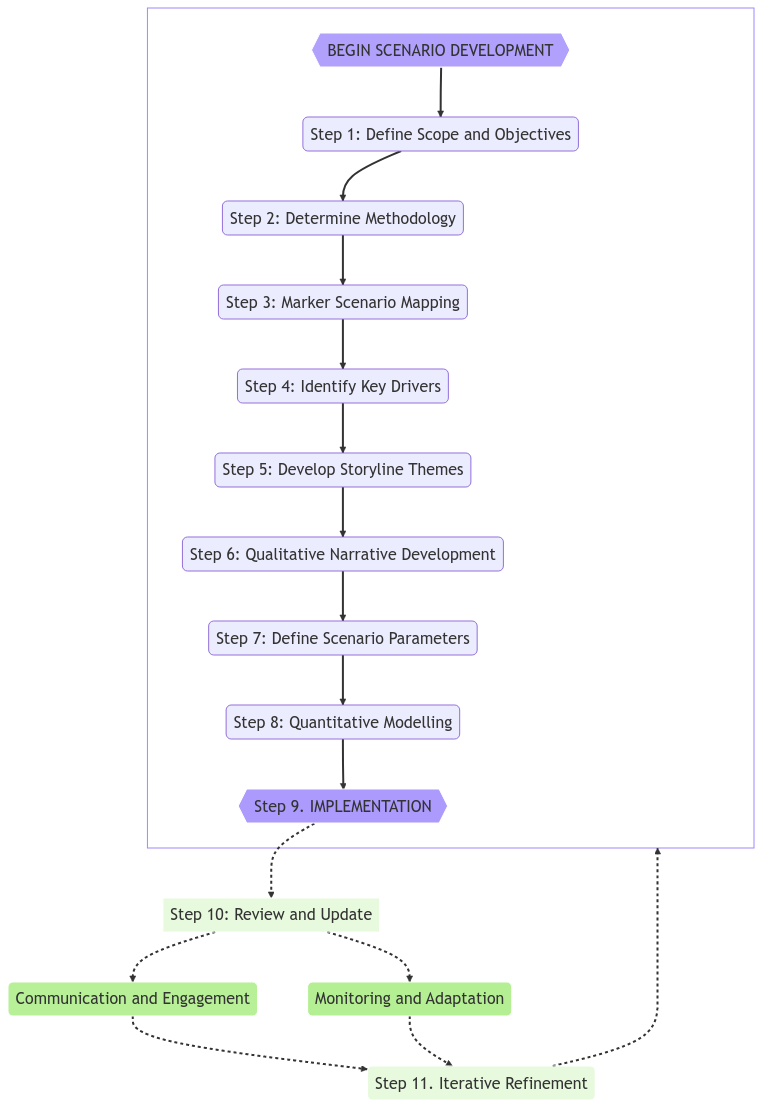
\includegraphics[width=\textwidth]{110methodology/fig_method.png}
  \caption{Scenario storyline development process}\label{fig:method}
\end{figure}



\subsection{Step 1: Define the scope and objectives}
\textbf{Scope and objectives of the scenario development process}

The scope and objectives of the scenario development process are defined in the context of the overall aim, scope, and objectives of the FutuRaM project.

\textbf{Aim of FutuRaM:}

FutuRaM will develop the Secondary Raw Materials knowledge base on the availability and recoverability of secondary raw materials (SRMs) within the European Union (EU), with a special focus on critical raw materials (CRMs). The project research will enable fact-based decision-making for the recovery and use of SRMs within and outside the EU, and disseminate the data generated via an accessible knowledge base developed in the project~\cite{futuram2022ca,futuram2022pmp}.

\textbf{Scope of FutuRaM:}

FutuRaM will establish a methodology, reporting structure, and guidance to improve the raw materials knowledge base up to 2050. FutuRaM will focus on six waste streams: batteries; electrical and electronic equipment; vehicles; mining; slags and ashes; and construction and demolition.

It will integrate SRM and CRM data to model their current stocks and flows and consider economic, technological, geopolitical, regulatory, social and environmental factors to further develop, demonstrate, and align SRM recovery projects with the United Nations Framework Classification for Resources (UNFC)~\cite{unfc2023}.

This will enable the commercial exploitation of SRMs and CRMs by manufacturers, recyclers, and investors, and the knowledge base developed in the project will support policymakers and governmental authorities.



Selected objectives of the FutuRaM project are presented in \autoref{tab:fm-objectives}~\cite{futuram2022ca,futuram2022pmp}.

\begin{table}[h!]
  \centering
  \small
  \caption{Selected objectives of the FutuRaM project}\label{tab:fm-objectives}
  \begin{tabular}{|L{7cm}|L{7cm}|}
    \hline
    \rowcolor{headerblue}\color{white}\textbf{NEED}                                                                                                                                                                                       & \color{white}\textbf{ACTION}                                                                                                                                                                                               \\
    \hline
    A successful transition to a climate-neutral, circular and digitised EU economy relies heavily on a secure supply of raw materials.                                                                                                   & FutuRaM will quantify the future availability of SRMs for three future scenarios for the EU material economy. \vspace{\baselineskip}
    Forecast material demand, SRM supply for each scenario, and raw material imports to evaluate EU material autonomy.                                                                                                                                                                                                                                                                                                                                                 \\
    \hline
    \rowcolor{fadedblue}
    Presently, several socioeconomic scenarios have been developed at national, EU, and/or global scales to assess the energy and mobility transition. \vspace{\baselineskip} Still lacking are specific scenarios for the SRM and CRM recovery systems & FutuRaM will develop stock-flow models for six waste streams based on holistic scenarios to map current and future material use in the economy of the EU-27 plus Iceland, Norway, Switzerland and the United Kingdom. \vspace{\baselineskip}
    FutuRaM will extend existing model approaches by a set of distinct scenarios that cover circular economy, high SRMs recoverability, and business as usual.                                                                                                                                                                                                                                                                                                        \\
    \hline
  \end{tabular}
\end{table}

\vspace{3em}

\textbf{Scope of Work Package 2 (WP2):}

Given this context, the scope of the scenario development process is to develop a set of plausible scenarios that explore the future of waste management, resource recovery, and circular economy in the EU.

The scenarios will be used to identify key drivers and uncertainties that will influence the future of waste management and resource recovery. The scenarios will also be used to evaluate the potential impacts of different policy interventions and technological advancements.


\textbf{\textit{Thematic scope}}

The scenarios will be centered on the six waste streams of FutuRaM:\@ WEEE, ELV, BAT, CDW, MIN, and SLASH.\ Additionally, consideration will be given to sectors and policy domains that are relevant to these waste streams and the general context of the system. These include manufacturing, energy, and transportation, as well as policies related to the environment, the economy, society, technology, and geopolitics.

\textbf{\textit{Geographic scope}}

The scenarios will be developed for the EU-27 plus Iceland, Norway, Switzerland and the United Kingdom (EU27+4). The scenarios will consider the current and future waste management practices and resource recovery technologies in these countries.
\vspace{\baselineskip}
Additionally, the scenarios will consider the current and future policies and targets related to waste management and resource efficiency in these countries. To some extent, the scenarios will also consider the current and future trade relationships between these countries and other countries around the world.

\textbf{\textit{Temporal scope}}

The scenarios will be developed for the time horizon of 2025--2050. This time horizon is aligned with the long-term targets of the EU, including the EU Green Deal, the EU Circular Economy Action Plan, and the EU Industrial Strategy.

The discrete stages in the forecasts are planned to be: 2025, 2030, 2035, 2040, 2045 and 2050.

The temporal resolution of the scenarios will be determined during the quantification phase of the scenario development process.

While it is possible to develop scenarios with a high (or even continuous) temporal resolution, that of these scenarios will be determined based on the availability and quality of data. It is important to acknowledge that providing too high a temporal resolution may lead to a false sense of accuracy and precision.

Furthermore, the scenarios will be developed with the understanding that the further into the future we look, the more uncertain the predictions become~\cite{amer2013,spaniol2017scenarios,kahn1967scenarios}.

\begin{table}[h]
  \textbf{WP2 --- Aims and objectives definition}
  \centering
  \small
  \caption{FutuRaM WP2 aims and objectives}\label{tab:fm-wp2objectives}
  \begin{tabular}{|L{7cm}|L{7cm}|}
    \hline
    \rowcolor{headerblue} \color{white}\textbf{AIM}                                                                                                                                           & \color{white}\textbf{OBJECTIVE}                                                                                                                                                                                                                                                                                                                                                                      \\ \hline
    Quantifying the current and future availability of secondary raw materials (SRM), particularly critical raw materials (CRM), for the identified waste streams from 2025 until 2050.       &
    Developing a set of plausible scenarios that encompass these waste streams and provide quantitative estimates of the current and future availability of SRM and CRMs.                                                                                                                                                                                                                                                                                                                                                                                                                            \\
    \hline
    Informing private and public sector decision-making processes by assessing the impacts of different legislative and policy strategies related to waste management and resource efficiency & The scenarios will cover a range of such strategies, grouped in coherent sets in each of the three storylines including recycling, reuse, remanufacturing, and landfilling. \newline Integration of the scenario with the system model will allow assessment of the impacts of these strategies not only on the availability of SRM and CRMs, but also on the environment, the economy, and society. \\
    \hline
  \end{tabular}
\end{table}



\subsubsection{Consideration of EU legislation and policy targets}\label{sec:legislation}

The scenarios developed in FutuRaM consider targets that the EU is setting for specific elements, materials, and waste streams. The targets incorporated into FuTuRaM's scenarios are aligned with the ambitions of the EU's Green Deal~\cite{eu2019greendeal} and its Critical Raw Materials (CRM) act~\cite{eu2023crmact}.

Additionally, the consumer-product-centric waste streams BATT, ELV, and WEEE have specific EU legislation that is directly applicable to them and will be considered in detail in the scenarios~\cite{eu2003weee,eu2012weee,eu2012weeerecast,eu2023elv,eu2023batt,eu2020batt}.

\textsc{General policies and legislation}

\textbf{The EU Green Deal}~\cite{eu2019greendeal} is a set of policy initiatives by the European Commission with the overarching aim of making the EU climate-neutral in 2050.

This policy portfolio is a response to the Paris Agreement and the United Nations Sustainable Development Goals. It covers a wide range of economic sectors with an emphasis on investments towards building local, 'sustainable' industries.

The scope of FutuRaM is aligned with the EU Green Deal's goal of ensuring the sustainable sourcing and use of raw materials, reducing dependency on imports, and promoting resource security. These goals can conflict with each other; however, the modelling in FutuRaM will explore the trade-offs between them (e.g., optimising local sourcing may result in higher negative externalities).



\textbf{The EU Circular Economy Action Plan}~\cite{eu2020circ} is a policy framework developed by the European Commission to promote the circular economy in the European Union.

It sets out a comprehensive set of measures and targets to improve resource efficiency, reduce waste, and foster sustainable production and consumption. The Action Plan includes initiatives related to product design, waste management, recycling, and resource efficiency, among others. The Action Plan is a key element of the European Green Deal and is closely linked to the EU Industrial Strategy.



\textbf{The Circular Economy Action Plan}:
\begin{itemize}
  \item Aims to promote the transition to a more circular economy in the EU.
  \item Sets out a range of measures to promote the sustainable use of resources, reduce waste, and increase recycling.
  \item Includes proposals for new legislation, such as an EU-wide framework for the circular economy, and revisions to existing legislation, such as the WEEE Directive.
  \item Emphasises the importance of product design for the circular economy and proposes measures to promote eco-design and repairability.
  \item Includes initiatives to promote the use of secondary raw materials, such as the establishment of a European Raw Materials Alliance.
  \item Aims to reduce greenhouse gas emissions and improve resource efficiency in the EU.
  \item Calls for increased cooperation and dialogue among stakeholders in the circular economy.
\end{itemize}



\textbf{The Critical Raw Materials Act} (CRM Act)~\cite{eu2023crmact} is an EU regulation that aims to ensure a secure and sustainable supply of raw materials to the EU.

The Act identifies a list of strategic raw materials, which are crucial to technologies important to Europe's green and digital ambitions and for defence and space applications, that are subject to potential supply risks. The regulation will cover the entire raw materials value chain, from primary extraction to manufacturing to potential recovery as a secondary raw material.

For example: According to the CRM act, by 2030, a single `third country' (ex-EU, ex-Schengen) should produce no more than 65\% of the EU's annual consumption of each strategic raw material.

Clear benchmarks have been set for the domestic capacities of the EU in 2030:
\begin{itemize}
  \item Extract at least 10\% of the EU's annual consumption
  \item Process at least 40\% of the EU's annual consumption
  \item Recycle at least 15\% of the EU's annual consumption
\end{itemize}

These benchmarks have been included in the scenarios developed in FutuRaM. Specifically, in the \hyperref[sec:rec]{Recovery scenario (REC)}, where the emphasis is on the recovery of materials from waste streams, and the \hyperref[sec:cir]{Circularity scenario (CIR)} where the emphasis is on the implementation of 're-X' strategies, such as recycling, remanufacturing, and reuse.

Many of these targets, benchmarks and mandates --- despite being included in legislation --- are considered too optimistic to be included in the \hyperref[sec:bau]{Business-as-usual scenario (BAU)} as they often make expectations whose attainment is likely highly unrealistic without radical reform of the waste management system, For example, the targets in the Battery Act suggest near-complete recovery for several elements~\cite{eu2020batt}.



\subsubsection{Extent of policy and legislation inclusion in the scenarios}

The targets that result from the planned and ongoing review processes are non-negotiable and legally binding and thus should be incorporated into our scenarios. These targets, however, are only applicable to post-consumer products, namely WEEE, BAT and ELV.\@ This envisioned future in which legally binding targets for collection, reuse and/or material recycling are achieved can be implemented as the Recovery scenario.

If there are no targets set for a specific consumer product category, then approach targets similar to the WEEE directive and in line with the EU Green Deal. For the Recovery, and especially for the Circularity scenario, FutuRaM will also consider the effects of proposed ecodesign requirements for sustainable products (e.g., longer lifetimes, increased reusability, repairability, recyclability).

However, for waste that does not consist of discarded consumer products, but instead results from industrial production activities, in particular for MIN and SLASH, we must still produce specific scenarios related to mining, metallurgy, and waste and fuel combustion. The production of new mining wastes will depend on new local mining activity.

Predicted production in the EU until 2050 will be forecast (equally across the three scenarios) and the flows into the MIN waste stream can be calculated with the respective transfer coefficients. The recovery of historical MIN stock, which is a target of the CRM Act, should be modelled differently. It requires a hypothesis about the percentage of historical tailings recoverable by commodity and country.

The scenarios will account for increasing resource use effectiveness and production process efficiency thus indicating lower volumes and quality of generated production residues (both by-products and waste such as red mud, waste rock, slags, etc.) per unit of product (expressed either as product mass or product value), whether that product is a metal (e.g., a copper cathode), metal alloy (e.g., aluminium alloy n° 5183) or metal product (e.g., cold rolled stainless steel sheet).

Excepting the BAU storyline, WEEE, ELV, and BATT waste material recovery will follow the targets in the EU.\@

For SLASH and MIN, we will evaluate recent trends in waste generation and extract plausible ranges of generation toward 2050.

For CDW, embedded WEEE will follow EU targets, and bulk waste will incorporate storylines and scenarios that are congruent with predicted demolition rates (where renovation is the alternative emphasised in the CIR storyline).

Various drivers will be assigned to move between these ranges and will be key to the specific, harmonized storyline for the scenario. Finally, the targets and storylines will be aligned with assumptions on technology development.



\subsubsection{Consideration of geopolitical developments}

The storylines also attempt to consider geopolitical considerations and thus supply chain resiliency for satisfying the product demand in the scenarios. We must omit, however, possible changes in waste flow volumes and composition that could arise from any material supply constraints.

The reasoning for this is that it would needlessly confuscate the interpretation of the modelling results as the incertitude of these potentialities is very high and this realm is outside the scope of FutuRaM's mandate and expertise.


The most volatile aspect of the `criticality calculation' is the risk profile of the producing country. For many material-exporting nations, this is not something that can be reliably forecast, especially not over the next 30 years. Thus, it will be assumed that the growth in material demand for (among other needs) the energy and mobility transitions can be satisfied either by an increase in mining and metallurgy activities within the EU or by growing imports from raw material-producing countries outside the EU.\@

That is, if we go for increased domestic EU production to minimize geopolitical supply risk, it may indicate more EU production residue generation even under increased production efficiency and resource effectiveness. The increase of domestic industrial activity, as a response to an envisioned increased internal demand, supposes an equivalent rise of societal approval for mining and refining activities on EU territory.

If the increased demand is, however, satisfied by imports from non-EU countries, which we know have domestic resource consumption also growing significantly due to the energy and mobility transition, our assumption would be to shift the mining and refining activities from EU countries towards resource-rich non-EU countries.


This shift would also imply an increased risk for geopolitical instability and/or security of supply of critical raw materials to the EU.

This situation is front of mind for many in policy and business and the EU is `applying a policy mix that aims to increase domestic capacity, diversify suppliers, and support the multilateral rules-based trade environment.`

However, `\ldots most experts predict that reshoring or nearshoring will be of limited importance. With time, though, resilience may improve through international cooperation, diversification and the accelerated uptake of digital technologies.'~\cite{szczepanski2021resilience}

\textbf{Note: supply constrictions will be considered in the model's sensitivity analysis and the codebase will be designed to allow for the optimisation of the SRM recovery system based on any value statements (such as profit, environmental impacts, supply and demand).}



\subsection{Step 2: Determine methodology}

\subsubsection{Methodology types and selection criteria}
The second step in the scenario development process is to determine the methodology to be used. This involves identifying the most appropriate methods and tools for the specific context and objectives of the scenario development process. The methodology should be selected based on the following criteria:

\begin{description}
  \item[\textbf{Relevance:}]
        The methodology should be relevant to the specific context and objectives of the scenario development process.
  \item[\textbf{Applicability:}]
        The methodology should be applicable to the specific context and objectives of the scenario development process.
  \item[\textbf{Feasibility:}]
        The methodology should be feasible given the available resources (e.g., time, budget, expertise, data, etc.).
  \item[\textbf{Transparency:}]
        The methodology should be transparent and well-documented, allowing for replication and further analysis.
  \item[\textbf{Flexibility:}]
        The methodology should be flexible and adaptable, allowing for updates and adjustments as new information becomes available.
  \item[\textbf{Accessibility:}]
        The methodology should be accessible to a wide range of stakeholders, ensuring that it can be understood and used by non-experts.
  \item[\textbf{Effectiveness:}]
        The methodology should be effective in achieving the objectives of the scenario development process.
  \item[\textbf{Efficiency:}]
        The methodology should be efficient in terms of time, cost, and resources required to implement it.
  \item[\textbf{Acceptability:}]
        The methodology should be acceptable to stakeholders, ensuring that it is perceived as fair and legitimate.
\end{description}


Further details are given in this section, and the table in \autoref{appendix:methods} provides an overview of the methods and tools considered, along with a brief description of each and its relevance to the specific context and objectives of the FutuRaM scenario development process.

\subsubsection{Choice of methodology}
The grant proposal for the FutuRaM project outlined that there should be at least three scenarios developed, namely business as usual, recovery, and circularity. This remains the case; however, during the scenario development process, additional scenarios or scenario dimensions were considered, including supply chain security and the energy transition.


\textbf{Considered dimension --- Supply chain security:}

Due to various political developments in 2022, the question of the security of the EU's supply chains for CRMs was brought into focus. This led to the proposal from stakeholders to consider a scenario dimension that would explore the security of the EU's supply chains for CRMs.


\textbf{Considered dimension --- Energy transition:}

The energy transition is a key topic in the EU's policy agenda, and the FutuRaM project is concerned with the role of CRMs in the energy transition. Therefore, the proposal was made to consider a scenario dimension that would explore the energy transition in the EU.\@


\textbf{Method --- Multi-criteria analysis and cross-impact analysis}

In order to assess the potential inclusion of these additional scenario dimensions, a multi-criteria analysis and a cross-impact analysis were conducted~\cite{steubing2016matrix}. The addition of extra dimensions increases the possible number of scenarios significantly. By assessing the consistency and plausibility of these combinations with a matrix-based method, it was possible to reduce the number of scenarios.

For example, low progress in the energy transition is unlikely to concur with high progress in recycling/circularity indicators and can be excluded. In contrast, different levels for the supply chain security dimension would result in an additional scenario, as this dimension is considered independent of the others.

Ultimately, supply chain security was eliminated as a scenario dimension. This is due to the consortium's inability to speculate on geopolitical developments and the added incertitude it would introduce to the scenarios.

The potential of supply constraints will, however, be considered in the future sensitivity analysis of the model, as well as potentially through an array of explorative multi-object optimisation procedures. This can produce projects to answer the question, `What would happen to the SRM system if element x is constrained, and what would be the optimal response to this constraint?'


\textbf{Method --- Delphi}

The Delphi method~\cite{hsu2019delphi} was used in the initial stages of the scenario-building process to gather and aggregate the opinions of experts or stakeholders. Internal consultation with consortium members who were experts in their respective waste streams or other aspects of the recovery system was conducted.

The method involves steps such as the selection of experts, generation of initial questionnaires, iterative rounds of responses, and convergence and consensus building. For the later stages of the process, further rounds of consultation will be conducted with external stakeholders, including representatives from industry, academia, and government.

\subsubsection{Choice of Scenario Type}
The general types of scenarios are summarized in \autoref{tab:scenario-types}. In the context of futures studies, various approaches and methodologies are employed to understand the potential trajectories of future developments~\cite{bishop2007scenarios,cordovapozo2023scenarios,skea2021outlooks,amer2013,boerjeson2005scenariosreport, boerjeson2005scenariosarticle}.

We can classify scenario studies into three primary categories, each addressing distinct questions about the future. These categories are tailored to better align with the specific objectives of scenario usage:

\vspace{2em}

{\large \textbf{Predictive Scenarios (Answering `What Will Happen?'):}}
\begin{description}[leftmargin=2cm]
  \item [\textbf{Pros}:] These scenarios offer insights into potential future outcomes, aiding in long-term planning.
  \item [\textbf{Cons}:] They are contingent on assumptions and may not account for unexpected events.
  \item [\textbf{Applicability}: ]Predictive scenarios are valuable when the aim is to forecast future developments under certain conditions.
\end{description}

{\large \textbf{Explorative Scenarios (Answering `What Can Happen?'):}}
\begin{description}[leftmargin=2cm]
  \item [\textbf{Pros}:] Explorative scenarios explore a wide range of potential future scenarios, fostering preparedness for various outcomes.
  \item [\textbf{Cons}:] They do not prioritize the likelihood or desirability of scenarios.
  \item [\textbf{Applicability}:] These scenarios are beneficial when considering multiple potential futures and the need to adapt to diverse outcomes.
\end{description}

{\large \textbf{Normative Scenarios (Answering `How Can a Specific Target Be Reached?'):}}
\begin{description}[leftmargin=2cm]
  \item [\textbf{Pros}:] Normative scenarios focus on achieving predefined objectives and offer guidance on strategies to attain them.
  \item [\textbf{Cons}:] They are inherently normative, starting with specific goals in mind.
  \item [\textbf{Applicability}:] Normative scenarios are suitable when the objective is to work towards predefined targets and develop actionable plans to reach them.
\end{description}

The choice of scenario category is influenced not only by the characteristics of the system under study but also by the user's worldview, perceptions, and study objectives. Additionally, the user's perspective plays a crucial role in determining the most suitable approach. For instance, the decision to employ predictive, explorative, or normative scenarios hinges on the user's goals and the nature of the questions they seek to answer.

Furthermore, considerations regarding the predictability of the future and the potential for influencing it can impact the selection of scenario types. For example, some users may argue that uncertainty in certain parameters makes long-term predictions less meaningful, while others may see value in using forecasting and optimisation models to stimulate discussions and inform decision-making processes.

In practice, a combination of qualitative and quantitative techniques can be employed to create scenarios tailored to specific needs. For instance, a blend of techniques may be used to generate forecasts, especially when external factors are uncertain. Likewise, strategic scenarios often begin with external scenario generation and proceed to identify available policy options.

\begin{landscape}
  \begin{table}[h]
  \centering
  \small
    \caption[Types of scenario]{Types of scenario (adapted from~\cite{boerjeson2005scenariosreport, boerjeson2005scenariosarticle})}\label{tab:scenario-types}
    \begin{tabular}{|L{4.5cm}|L{1.9cm}|L{4.5cm}|L{4.0cm}|L{2.2cm}|L{4.0cm}|}
      \rowcolor{headerblue}
      \hline
      \textcolor{white}{\textbf{SCENARIO CATEGORY}}                                     & \textcolor{white}{\textbf{SCENARIO TYPE}} & \textcolor{white}{\textbf{OUTCOME}}              & \textcolor{white}{\textbf{TIMEFRAME}} & \textcolor{white}{\textbf{SYSTEM STRUCTURE}} & \textcolor{white}{\textbf{FOCUS ON FACTORS}} \\
      \hline
      \multirow{2}{=}{\textbf{Predictive}\newline \textit{what will happen?}}           & Forecasts                                 & Typically quantitative, sometimes qualitative    & Often short                           & Typically one                                & Typically external                           \\
      \cline{2-6}
                                                                                        & What-if                                   & Typically quantitative, sometimes qualitative    & Often short                           & One to several                               & External and, possibly, internal             \\
      \hline
      \multirow{2}{=}{\textbf{Explorative}\newline \textit{what can happen?}}           & External                                  & Typically qualitative, quantitatively possible   & Often long                            & Often several                                & External                                     \\
      \cline{2-6}
                                                                                        & Strategic                                 & Qualitative and quantitative                     & Often long                            & Often several                                & Internal under influence of the external     \\
      \hline
      \multirow{2}{=}{\textbf{Normative}\newline \textit{how can a target be reached?}} & Preserving                                & Typically quantitative                           & Often long                            & One                                          & Both external and internal                   \\
      \cline{2-6}
                                                                                        & Transforming                              & Typically qualitative with quantitative elements & Often very long                       & Changing, can be several                     & Not applicable                               \\
      \hline
    \end{tabular}
  \end{table}
\end{landscape}



\textbf{The scenarios developed in the FutuRaM project are a combination of predictive and normative:}
\begin{description}
  \item[\iconBAU \textbf{BAU:}]
        \textit{What will happen if current trends continue?} 
        \vspace{0.5\baselineskip}
        This scenario is predictive in nature, based on the assumption that the current trends and developments in waste management and resource recovery systems will continue into the future.
  \item[\iconREC \textbf{Recovery:}]
        \textit{What will it take to achieve the EU's targets for material use and recovery? \\ Focus on technology} 
        \vspace{0.5\baselineskip}
        This scenario is normative, focusing on manipulating the technology and infrastructure of the recovery system to achieve the EU's targets and mandates.
  \item[\iconCIR \textbf{Circularity:}]
        \textit{What will it take to achieve the EU's targets for material use and recovery? \\ Focus on re-X strategies} 
        \vspace{0.5\baselineskip}
        This scenario is a combination of normative and explorative, considering the targets and mandates of the EU's circular economy action plan and exploring re-X strategies in the recovery system.
\end{description}

The methodology and scenario types were selected based on their relevance, applicability, feasibility, transparency, flexibility, accessibility, effectiveness, efficiency, and acceptability to the scenario development process.



\subsection{Step 3: Marker-scenario mapping}

\subsubsection{Justification and methodology}
This preliminary step in the scenario development process involves conducting a literature study to identify existing scenarios that are relevant to the FutuRaM project. This step is crucial as it serves several important purposes and provides valuable insights for the overall scenario development process. It helps the scenario development team to build on existing knowledge, identify relevant scenarios, gain insights and inspiration, fill knowledge gaps, and enhance credibility and comparability.



\textbf{Building on existing knowledge}\\
Conducting a literature study allows the FutuRaM project team to tap into existing knowledge and expertise in the fields of waste management, resource recovery, and circular economy. It provides a foundation of existing scenarios that have been developed by other researchers, organizations, or institutions. By building on this existing knowledge, the FutuRaM project can leverage the insights, methodologies, and findings from previous scenario studies, saving time and resources.



\textbf{Identifying relevant scenarios}\\
Marker scenario mapping helps identify scenarios that are relevant to the specific objectives and scope of the FutuRaM project. By reviewing the literature, the project team can assess the applicability of existing scenarios to their research questions and determine which scenarios align with the waste streams, sectors, and policy domains being considered. This step ensures that the scenarios selected for further analysis are well-suited to address the project's goals.



\textbf{Gaining insights and inspiration}\\
Reviewing existing scenarios provides the FutuRaM project team with valuable insights and inspiration for the development of their own scenarios. It allows them to understand the different approaches, assumptions, and methodologies used in previous scenario studies. This knowledge can inform the design and structure of the FutuRaM scenarios, helping to ensure a rigorous and well-founded approach.



\textbf{Filling knowledge gaps}\\
Marker scenario mapping helps identify any gaps or areas of limited knowledge in the existing scenario landscape. It allows the FutuRaM project team to identify topics or aspects that have not been adequately addressed in previous scenarios. This awareness of knowledge gaps can guide the project team in focusing their efforts on areas where new insights and contributions can be made, leading to a more comprehensive and innovative scenario development process.



\textbf{Enhancing credibility and comparability}\\
By conducting a literature study and referencing existing scenarios, the FutuRaM project can enhance the credibility and comparability of their own scenarios. The project team can reference and compare their findings, assumptions, and results with those from previous studies, contributing to the overall body of knowledge in the field. This promotes transparency, robustness, and consistency in the scenario development process and allows for better benchmarking and evaluation of the FutuRaM scenario set.



\subsubsection{Content of the marker scenario mapping for application to FutuRaM's scenarios}

\autoref{tab:marker-scenarios} in \autoref{appendix:marker-scenarios} presents an overview of the marker scenarios considered in the FutuRaM project. The table is not intended to be exhaustive but rather to provide an overview of the different scenarios that have been developed in the fields of waste management, resource recovery, and circular economy.



\subsection{Step 4: Identification of key drivers of change}

In this step, the key drivers of change that will shape the future of the scenarios are identified. Key drivers are the factors or forces that have a significant influence on the waste management system and its development over time. These drivers can be social, economic, technological, environmental, or policy-related.

The purpose of identifying key drivers of change is to understand the factors that will have the greatest impact on waste management and to ensure that the scenarios capture the range of possible outcomes influenced by these drivers.

The process of identifying key drivers involves a combination of literature review, expert consultations, and stakeholder engagement. It requires a comprehensive analysis of relevant trends, uncertainties, and emerging issues that may affect the waste management system.

The key drivers identified in this step will be used to develop the storyline themes and scenario parameters in the next step.

\autoref{fig:screening-method} illustrates the process of identifying key drivers of change.

\begin{figure}[h!]
  \centering
  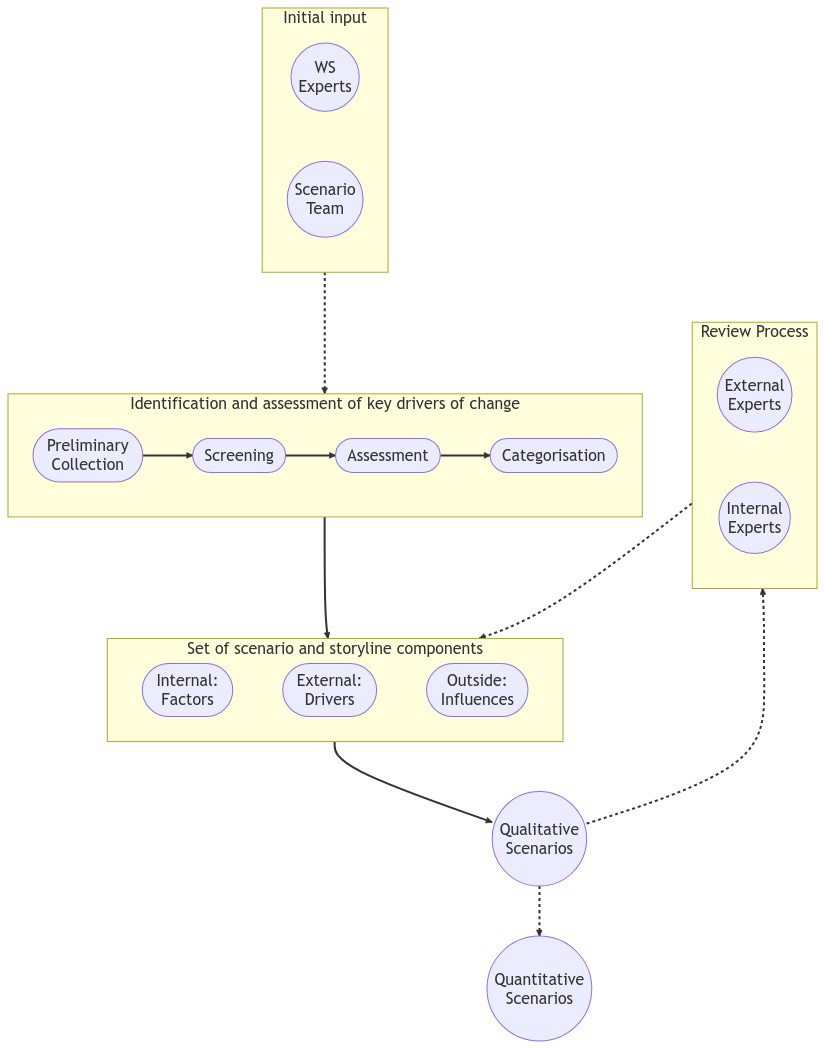
\includegraphics[width=1\textwidth]{110methodology/figure_screeningmethod.png}
  \caption{An illustration of the process used for identifying key drivers of change}\label{fig:screening-method}
\end{figure}
\clearpage



\subsubsection{Methodology and results of this stage in FutuRaM's scenario development:}

The overall goal of this process is to identify and include elements in the storylines and scenarios that are relevant, plausible, and influential in shaping the future.

The selection, screening, and categorisation steps ensure that the elements chosen for the development of storylines and scenarios are consistent, coherent, and aligned with the objectives and scope of the scenario exercise.

\begin{enumerate}
  \item \textbf{Preliminary collection:}

        This step involved gathering a pool of potential elements that could be included in the storylines and scenarios.


        These elements were derived from expert input from waste streams and the scenario development team, including taking knowledge from the literature review and existing scenarios identified in Step 2 --- Marker scenario mapping.
        \vspace{\baselineskip}

        This step was conducted using the PESTLE analysis framework. The PESTEL (or PESTLE) framework is a strategic tool used to understand the macro-environmental factors that can affect a system.

        A PESTEL analysis can help identify opportunities and threats linked to each of these factors, understand the broader context, and shape scenarios accordingly~\cite{kokkinos2023methodspestel,sansa2021methodspestel}.

        \vspace{\baselineskip}

        \textbf{The acronym PESTEL stands for:}

        \begin{description}[style=nextline]

          \item [\textbf{Political}:]
                These factors refer to the impact of government policies, regulations, and political stability. This includes issues like tax policy, labour laws, environmental regulations, trade restrictions and reforms, tariffs, and political stability.

          \item [\textbf{Economic}:]
                These factors relate to the broader economic environment, including factors like economic growth, exchange rates, inflation rates, interest rates, disposable income of consumers and businesses, and the general health of the economy.

          \item  [\textbf{Sociocultural}:]
                These factors include societal trends and characteristics that could affect your business. They include demographic trends (like age, gender, and ethnicity), cultural trends, lifestyle preferences, consumer attitudes, and broader societal expectations.

          \item  [\textbf{Technological}:]
                These factors refer to the impact of emerging technologies, research and development activities, automation, the rate of technological change, and the adoption of technology within your market.

          \item  [\textbf{Environmental}:]
                These factors refer to ecological aspects that can affect a system. This includes environmental regulations, consumer attitudes towards sustainability, climate change, and other natural events.

          \item  [\textbf{Legal}:]
                These factors include laws and regulations with which your business must comply. These can include labour law, consumer law, health and safety law, and restrictions on the import or export of goods.

        \end{description}

        \vspace{\baselineskip}
        \textbf{The 68 elements identified in the initial screening stage are listed in \autoref{appendix:elements-1}.}

        \vspace{\baselineskip}

  \item \textbf{Screening:}

        In the screening step, the collected elements are evaluated and assessed based on specific criteria. This was conducted through a literature study and internal consultation of scientists in the project. This evaluation helps determine the relevance, reliability, and significance of each element for the development of storylines and scenarios. Many elements were aggregated, especially if they were deemed to follow similar trends to others (e.g., recyclability mandates and improved recyclability in project design). Elements that did not meet the predefined criteria or were deemed irrelevant, `un-modellable' or unreliable were excluded from further consideration (e.g., corruption, data protection, and supply chain conflict).

        \vspace{\baselineskip}

        The 28 elements that were identified in this stage are listed in \autoref{appendix:elements-2}.

        \vspace{\baselineskip}

        In \autoref{fig:screening-exercise}, an excerpt of a spreadsheet illustrates part of the screening process for the FutuRaM scenarios, which was informed by the waste streams. In this exercise, the elements were evaluated based on their relevance to the waste streams and their potential impact on the waste management system.
        
        The elements were also assessed based on their plausibility and likelihood of occurrence in the future. The elements that were deemed relevant, plausible, and influential were included in the storylines and scenarios.

        \begin{landscape}
          \begin{figure}[h]
            \centering
            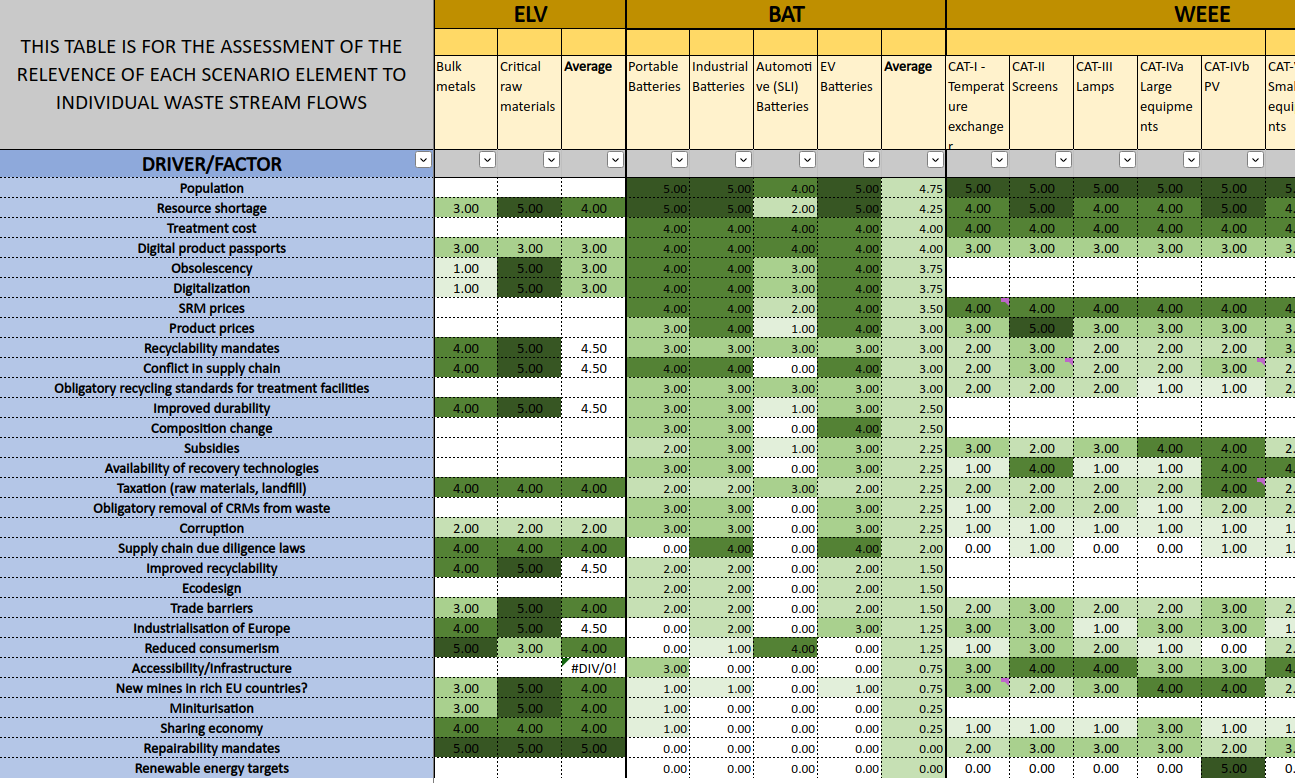
\includegraphics[width=\linewidth]{110methodology/figure_screeningexercise.png}
            \caption{An excerpt of a spreadsheet used as part of the screening process}\label{fig:screening-exercise}
          \end{figure}
        \end{landscape}



  \item \textbf{Assessment:}

        Once the screening process was complete, the remaining elements were aggregated and categorized based on their thematic relevance or characteristics. This categorisation helps organize the elements into meaningful groups or themes that align with the objectives and scope of the scenarios.
        \vspace{\baselineskip}
        The 21 elements that were identified in this stage are listed in \autoref{tab:keydrivers}. Note that CIR and REC are very similar for many scenario elements, the main difference being the way in which the targets are achieved. That is, for CIR, re-X strategies are promoted, whereas, for REC, the focus is on technological advancements in the recovery system. This distinction will have a significant impact on how the scenarios are quantitatively modelled and on the subsequent outcomes of these models.

        \begin{landscape}
          \small
          \begin{longtable}{|L{1.5cm}|L{7cm}|L{9cm}|L{1.5cm}|L{0.5cm}|L{0.5cm}|L{0.5cm}|}
            \caption{List of drivers and factors identified in the screening phase}\label{tab:keydrivers}                                                                                                                              \\
            \hline
            \rowcolor{headerblue}
            \color{white}\textbf{DOMAIN} & \color{white}\textbf{DRIVER/FACTOR} & \color{white}\textbf{DEFINITION} & \color{white}\textbf{INTERNAL} & \color{white}\textbf{BAU} & \color{white}\textbf{REC} & \color{white}\textbf{CIR} \\
            \hline
            \endfirsthead%
            \hline
            \multicolumn{7}{r}{\color{headerblue}{\textit{{Continued on next page}}}}                                                                                                                                                  \\
            \endfoot%
            \rowcolor{white}
            \multicolumn{7}{c}{{\color{headerblue}{\textit{\tablename\ \thetable{} --- Continued from previous page}}}}                                                                                                                \\
            \hline
            \rowcolor{headerblue}
            \color{white}\textbf{DOMAIN} & \color{white}\textbf{DRIVER/FACTOR} & \color{white}\textbf{DEFINITION} & \color{white}\textbf{INTERNAL} & \color{white}\textbf{BAU} & \color{white}\textbf{REC} & \color{white}\textbf{CIR} \\
            \hline
            \endhead%
            \bottomrule
            \endlastfoot%
            \csvreader[late after last line=\ , separator=semicolon]{csvs/elements-3.csv}{}{
            \csvcoli                     & \csvcolii                           & \csvcoliii                       & \csvcoliv                      & \csvcolv                  & \csvcolvi                 & \csvcolvii                \\
            }
          \end{longtable}
        \end{landscape}



  \item \textbf{Categorisation}

        The scenario elements were then assessed based on their potential impact on the waste management system. For each element, an assessment was made as to whether it was within the scope of FutuRaM to include them as variables in the models, and therefore also the scenarios and their storylines.

        \vspace{\baselineskip}

        Those deemed to be within the scope are `internal' and will be intensively researched and modelled (e.g., composition and design changes).

        \vspace{\baselineskip}

        Those deemed to be outside the scope are `external' and will be included in the storylines, will vary over time, but will not vary across the three scenarios (e.g., population and GPD).

        \vspace{\baselineskip}

        Those deemed to be outside the scope and also outside the influence of the waste management system are `outside' and will not be included in the storylines or scenarios, though, in some cases, may be considered in the sensitivity analysis (e.g., supply constraints).


        \subsubsection{Justification for keeping certain elements outside of the scenario models:}

        The purpose of the FutuRaM project is not to provide all-encompassing scenarios that attempt to capture every possible future development. Such scenarios are inherently inaccurate and can give a false sense of certainty to the model's outcomes. Instead, the focus of FutuRaM is specifically on the Sustainable Resource Management (SRM) system and its implications for the future. Therefore, the scenarios developed within FutuRaM should selectively incorporate elements that have a direct impact on the SRM system.
        \vspace{\baselineskip}

        Furthermore, the scenarios should prioritize elements that can be considered as `policy knobs', meaning variables or factors that can be adjusted or controlled to test different settings. By including these, the scenarios can explore the effects of different policy decisions or interventions on the SRM system's outcomes. This targeted approach ensures that the scenarios generated are relevant to the project's objectives and facilitate meaningful analysis.
        \vspace{\baselineskip}

        It is crucial to avoid excessive complexity and convolution in scenario modelling. When there are too many convoluted elements included, the results of the modelling exercise can become, at best, difficult to understand and interpret. At worst, the outcomes may become practically useless due to the overwhelming interactions and uncertainties introduced by the complex elements. Therefore, careful consideration is necessary to strike a balance between incorporating essential factors and maintaining the clarity and usefulness of the scenario modelling results.

        \subsubsection{Examples:}

        \begin{description}[style=nextline]

          \item [\textbf{Resource shortages:}]
                Resource shortages can be highly unpredictable and subject to various external factors such as geopolitical events, natural disasters, or technological advancements. The precise timing and extent of resource shortages are challenging to forecast accurately, making it difficult to include them within the model without introducing significant uncertainty.\\
                This is especially true for the long-term time horizon of the FutuRaM scenario set. This factor will, however, be considered in the sensitivity analysis of the model and additionally, the codebase will be designed to allow for the optimization of the SRM recovery system based on any supply-demand value statements.

          \item [\textbf{Raw material vs SRM prices:}]
                The dynamics and competition between raw materials and secondary raw materials can be complex and influenced by various market factors, technological advancements and policy interventions.
                As with resource shortages, these dynamics are challenging to forecast accurately, making it difficult to include them within the model without introducing significant uncertainty.\\It will, however, be possible to couple the model with a market model to explore the effects of different price dynamics on the SRM system's outcomes. This could be considered in a multi-objective optimization procedure performed as an extension to the model.

        \end{description}

\end{enumerate}



\subsection{Step 5: Develop storyline themes}

Given that the scenario themes and directions were broadly dictated by the FutuRaM project charter, the rough shapes of the storyline narratives were already defined. That is: the effects on the availability of SRMs from the development of the SRM recovery system and the development of re-X strategies.

\vspace{\baselineskip} 

\subsection{Step 6: Qualitative narrative development}

The scenario storylines will be described in detail in the next section. This step involved taking the themes defined by the charter and the elements identified in the previous steps and working with the internal waste stream groups to develop qualitative estimates about how each of these elements (at their different levels) may have an impact on the amounts and composition of the SRM flows in their purview.

\vspace{\baselineskip} 

\subsection{Step 7: Definition of scenario parameters}

The scenario parameters are the set of quantitative values or functions that will be used to define the scenario inputs for the model. Details of these parameters can be found in \autoref{chapter:quantification}.

\vspace{\baselineskip} 

\subsection{Step 8: Quantitative modelling}

Full details of the scenario quantification process can be found in \autoref{chapter:quantification}.

\vspace{\baselineskip} 

\subsection{Step 9: Implementation}

The scenario implementation will be performed in the next stages of the project.

\vspace{\baselineskip} 

\subsection{Step 10: Review process}

The review process is intended to ensure that the elements included in the storylines and scenarios are relevant, plausible, and consistent with the scenario objectives and scope.

The first stage of the review process is to open the scenario development process to the wider FutuRaM consortium. This will be done by sharing the scenario development process and the results of the assessment and categorisation step with the consortium and inviting feedback and suggestions. The feedback will be used to refine the elements and their categorisation and to identify any elements that may have been missed in the initial assessment.

The second stage will involve opening the scenario development process to external stakeholders and subject matter experts.

The scenario review process will be performed repeatedly over all stages of the project. This document is a living document and will be updated as the project progresses.

\subsubsection{Conclusion of methodology section}

The methodology used for the FutuRaM scenario development ensured that the selected elements were relevant, plausible, and influential. The use of the PESTEL analysis framework and Delphi method during the preliminary collection phase provided a comprehensive overview of the macro-environmental factors.

Furthermore, the screening process and the assessment by internal experts ensured that the selected elements were coherent, consistent, and aligned with the objectives and scope of the scenario exercise.

The final list of scenario elements is suited to the goal of the FutuRaM project --- to quantify the future availability of SRMs and to evaluate EU material autonomy ---  and will be used to develop the three FutuRaM scenarios into a quantitative model.


% end of chapter
\chapterEndlines
